\documentclass[12pt,a4paper]{report}

\usepackage[utf8]{inputenc}
\usepackage{graphicx}
\usepackage[square,sort,comma,numbers]{natbib}
\usepackage{gantt}
\usepackage{pdflscape}
\usepackage{datetime}

\newdate{date}{21}{06}{2017}

\begin{document}
\begin{titlepage}
	\centering
	
    %{\scshape\LARGE Candidature Assessment Report \par}
	%\vspace{2cm}
	
    {\huge\bfseries Localization And Mapping On An Agile Robot Platform\par}
	\vspace{2cm}
	
    {\Large\bfseries Janindu Arukgoda\par} 
    {\Large Centre for Autonomous Systems\par}
    {\Large Faculty of Engineering \& Information Technology\par}
    {\Large University of Technology Sydney\par}
    \vspace{1cm}
    
    {\large\texttt{janindusithumini.arukgoda{@}student.uts.edu.au}}
    \vspace{1cm}
    
    {\Large Principal Supervisor: Prof. Gamini Dissanayake\par}
    {\Large Co-Supervisor: Dr. Ravindra Ranasinghe\par}
	{\vfill}
    
	{\large Wednesday 21\textsuperscript{st} June, 2017 \par}
\end{titlepage}

%Abstract
\begin{abstract}
\par Robots are being used increasingly in place of humans where it is safer or more efficient alternative. Demolition sites and disaster struck buildings are two indoor environments where autonomous robots are preferred over humans. 

\par For decision making on how to proceed, the demolition crews and first responders to disasters need to inspect the affected environments. As time is of the essence, a fast and agile robot offers a significant advantage in such situations. While a camera mounted on a robot can provide visual information for the demolition crews or the first responders, a persistent representation of the environment is better suited for this job. 3-D reconstruction and mapping algorithms have been tried and tested on various conditions in many scenarios. However, most of the algorithms available are likely to fail.  
% * <ravindra.ranasinghe@uts.edu.au> 2017-06-19T06:52:11.208Z:
% 
% > However, most of the algorithms available are likely to fail.
% Perhaps you need to mention in few words why these algorithms are likely to fail.
% 
% ^.

\par In this research we propose a novel, agile robot platform that can navigate in such cluttered indoor environments and complement it with a mapping and localization strategy, giving it the capability to explore the environment fully autonomously with the aim of providing demolition crews and first responders to disasters with a fully functional autonomous robot platform. 

\end{abstract}

%Table of content
\tableofcontents

%Introcution
\chapter{Introduction}

\section{Background and Motivation}
\label{background}
With the advancements of technology, humans have continuously developed safer and more efficient alternatives to replace themselves. Robots are a popular alternative when it is unsafe for humans to operate in an environment. Both autonomous and remotely controlled robots are used to navigate in environments where the humans can't safely reach and execute tasks ranging from generic tasks such as observing and mapping the surroundings to more specific tasks such as pushing a button to shutdown a system. \par

Demolition sites and disaster struck buildings are two examples for such unsafe indoor environments. However, wheeled robots and humanoid robots face difficulties in navigation due to the unstructured and cluttered nature of the environment. Micro aerial vehicles such as quadrotors have more freedom navigating in these types of environments although the traditional quadrotor platform cannot be expected to survive even the slightest of collision against a structure. We plan to develop an agile quadrotor platform that can overcome this limitation of the traditional quadrotor platform which will enable it to successfully navigate in cluttered indoor environments such as aforementioned demolition sites and disaster struck buildings. \par 

Often, the demolition crews or the first responders to disasters need to inspect the affected area to make decisions on how to proceed. It is desirable for a robot to have capabilities above a simple camera feed to represent the environment. Current technology has produced mapping algorithms that have successfully been used on wheeled mobile robots and micro aerial vehicles to build various types of maps ranging from feature based maps to grid based maps to dense representation to sparse representation \cite{WURM2010140,grzonka2012fully,Cadena2016,g2oKummerle2011,ila2010,doi:10.1177/0278364914523689}. We anticipate to develop a novel environment representation method  specifically considering the limitations of the agile quadrotor platform such as the sensors attached to it as well as the platform dynamics and the constraints it operates under. \par 

The representation of the environment (map) can be either built by navigating the quadrotor platform manually or allowing it to navigate autonomously. Allowing the platform to navigate in autonomy during the mapping mission is more efficient in terms of complete area coverage given the unstructured and cluttered nature of the environments such as demolition sites and disaster struck buildings. Given the unique capabilities of the platform, we plan to come up with a simple and platform specific approach for autonomous exploration of cluttered indoor environments.

\section{Research Objectives and Methodology}
\label{researchObjectives}
In this subsection, the scope of the research is dissected into three main topics. The final objective of the research is to produce an agile quadrotor platform that can navigate in cluttered indoor environments for inspections. Each topic covers a core component of the research and aims to produce a key contribution that will lead to accomplish the the end goal. \par

\begin{itemize}
	\item\textbf{Agile Quadrotor Platform Design}
    \\Under this topic, we aim to design an agile quadrotor platform that can navigate in cluttered and unstructured indoor environments. The standard quadrotor platform architecture is not robust against collisions. In cluttered indoor environments, colluding against surfaces is to be expected. We try to address this problem by adding a light weight two wheeled cage around the quadrotor. Apart from robustness against collisions, we also hope to give the platform the capability to roll on surfaces at any angle, giving it much improved maneuverability. Furthermore, we plan on investigating control strategies to develop a simple yet novel approach to control the platform. \par
    \textbf{\emph{Contribution:}} 
    An agile quadrotor platform that can fly around and roll on surfaces in cluttered indoor environments and a strategy to control it.
        
    \item\textbf{Distance Function Based Outdoor Mapping And 6-DOF Localization in 3-D Environments}
    \\Distance function based environment representation has been used to map environments in 2-D using wheeled robots \cite{dantanarayana2016navigation}. Micro Aerial Vehicles move in 3-D space. We will examine how a similar approach based on distance functions can be used to represent the environment in 3-D  that can be used by a 6-DOF localizer so that an autonomous navigation system can be implemented on a Micro Aerial Vehicle platform. \par

    \textbf{\emph{Contribution:}}
    A 6-DOF localizer for Micro Aerial Vehicles that is based on a distance function based 3-D representation of the world. 
% * <ravindra.ranasinghe@uts.edu.au> 2017-06-14T22:30:39.509Z:
% 
% >  A 6-DOF localizer for Micro Aerial Vehicles that is based on a distance function based 3-D representation of the world. 
% 
% 
% This is not right. I think firstly you need to built distance based map using proper SLAM. The 6DOF localiser is the one which we've come up with for the MBZIRC competition. Whether we further improve this based on  a proper map with uncertainties is another question. Can you pls. check more on this with Dissa?  
% 
% ^.
    
% * <ravindra.ranasinghe@uts.edu.au> 2017-06-14T22:34:42.180Z:
% 
% Regarding my previous note:
% I think you better move the environment representation section above the 6DOF localiser section.
% In the second point in topic sentence you mentioned that "Distance Function Based Outdoor Mapping and 6-DOF Localization". However the text mainly focus on the localisation. My feeling is tha you describe mapping in one point and localisation in another.
% 
% Pls. have a good chat with Dissa on this. 
% 
% ^.    

	\item\textbf{Representation Of Unstructured, Cluttered And Dynamic Indoor Environments}
    \\Here we focus on mapping the cluttered 3-D indoor environment observed while navigating through it.  Given the payload capacity limit of micro aerial vehicles, the sensors that can be attached are limited. We plan to incorporate the platform dynamics and the constraints it operates under to the sensory information obtained to produce a dense 3-D map of the environment. We will mainly focus on a computer vision based approach using sensors like monocular and stereo cameras and inertial measurement units. We expect to build up on our work on 6-DOF outdoor localization and represent the map using distance functions. \par
    \textbf{\emph{Contribution:}}
    A SLAM algorithm that can exploit the platform specific motion constraints to obtain a dense 3-D map of a cluttered environment.
    
    \item\textbf{Exploration Of Unstructured, Cluttered And Dynamic Indoor Environments}
    \\Given the agile quadrotor platform with a control strategy, a mapping and localization system and a sensor setup, we hope to investigate for an appropriate exploration strategy to give the platform true autonomous navigation capability. The capability of the platform to roll on surfaces at any angle allows it to follow trajectories that are infeasible for the traditional wheeled robots and micro aerial vehicles allowing it to perform exploration of unknown environments in a novel way. \par 
    \textbf{\emph{Contribution:}}
    A platform specific exploration approach that allows the agile quadrotor platform to autonomously navigate in cluttered and unstructured indoor environments. 
    
\end{itemize}

%Literature Review
\chapter{Literature Review}

\section{Agile Robot Platforms}
\label{litWallClimbingRobots}
Wheel based ground robots vehicles such as Willow Garage\textregistered\ TurtleBot\texttrademark and CLEARPATH\texttrademark\ Robotics Husky are popular among researchers. While they can navigate in near horizontal flat terrains, they are not suitable for navigation in cluttered environments. Robots inspired by animals \cite{Lewinger2009}\cite{Parasuraman2010} and humans \cite{Kaneko2008} \cite{ROB:ROB21697} have been developed to navigate in more challenging terrains and even swim \cite{Nakashima2016}. However, these platforms do not have the capability to navigate along vertical and near vertical terrains.

Wall Climbing robots have been developed based on various principles. Adhesion based robots \cite{NISHI1992543} \cite{NISHI1986} and propulsion force based robots \cite{NISHI1991} have been proposed for wall climbing around three decades ago. The adhesion based wall climbing robots can be classified into four groups based on the adhesion method as magnetic, hand–hold, biologically inspired and vacuum suction pad \cite{Koo2013}. The main problem with these robots is that they need flat surfaces to adhere to, and obstacles such as grooves make it difficult to seal the suction \cite{Liu2013}. 

Quadrotors have been designed with a cage added around it both as a protective measure \cite{mulgaonkar2015design} \cite{sadeghzadeh2011fault} as well as to give it the terrestrial motion capability \cite{kalantari2013design}. A limitation of the latter system is that it has been modeled only for horizontal terrains. Parrot \textsuperscript{\textregistered} Minidrones Rolling Spider and Helic Max Sky Walker are two commercially available quadrotors which have this terrestrial motion capability due to wheels and a cylindrical cage respectively. For both aerial and terrestrial motion, these platforms use the same actuators. However, these products are remote controlled toys and neither they have the computational power on-board nor have the payload capacity to carry an additional computer to host an autonomous navigation system. However they have demonstrated the wall climbing capability. 

While the passive rotating spherical and cylindrical cages mentioned above allow the Micro Aerial Vehicles to navigate safely in cluttered and enclosed environments, it also makes physical interactions with the world hard. As mentioned in section \ref{background}, autonomous robots are needed to perform specific tasks, interacting with the world using manipulators. In the work described in section \ref{mbzircProgress}, a magnetic gripper was used to pick up objects. Salaan et al. \cite{salaan2017uav} presents a solution to this by implementing two-axis passive rotation with independent rotation of two hemispherical shells around a quadrotor. A gap unaffected by the independently rotating hemispherical shells is maintained along the roll axis to allow manipulators to be extended to interact with the world. A novel feedback control algorithm is proposed in \cite{wopereis2017application} for quadrotors with manipulators which allows applying large and continuous forces on external surfaces.  

\section{Simultaneous Localization And Mapping}
For a robot platform to have true autonomous navigation capability, it should be able to navigate in unchartered territory without any manual interventions. To this end, it has to build a knowledge base of the environment using only the relative observations that its exteroceptive sensors provide. This knowledge base of the environment is said to be the map of the environment. For navigation tasks such as path planning and obstacle avoidance, the robot should locate itself within this map, i.e. localization. In Simultaneous Localization and Mapping (SLAM), as the name suggests, both mapping and localization tasks are carried out in parallel. \par

In a very high level, the solutions to the SLAM problem can be classified by the techniques used to represent the map and to estimate the robot states. Occupancy Grid Maps (OGM) and landmark based maps are two such map representations used in the 2D case \cite{WURM2010140}. Since aerial vehicles navigate exciting full 6-DOF motion, a 3-D estimation of the pose is required. Modeling the 3D geometry is more complicated than the 2D case. Some approaches identified can be listed as (i) Landmark-based sparse representation, (ii) Low-level raw dense representation and (iii) Boundary and spatial-partitioning \cite{Cadena2016}. Landmark-based sparse representation is essentially the 3D counterpart of a landmark based map mentioned earlier. Lines, corners and curves are identified as features that describe the environment and those features collectively form the map. In the low-level dense representation, the environment is described using unstructured points or polygons. However, this requires comparatively larger storage. Boundary and spatial-partitioning dense representation attempts to represent surfaces of the environment instead of simply using point clouds. The advantage is that the topology of obstacles is not ignored.

Distance function based environment representation is also used with scan-to-map matching for map building. Chamfer Distance \cite{barrow1977parametric} and Hausdorff Distance \cite{huttenlocher1993comparing} are two popular template matching techniques. CD Mapping \cite{dantanarayana2016navigation} is a Chamfer Distance based scan-to-map matching technique for map building. Chamfer distance has also been used with OGM for localization \cite{dantanarayana2013c}.

The traditional approach to state estimation is the filter based approach \cite{Cadena2016}. Kalman filter and particle filter are two of the most widely used filter based approaches. Kalman filters are commonly used as a single step optimizer for robot state estimation with landmark / feature based maps \cite{SLAM_Dissa}. Particle filter is an iterative approach to the state estimation that is seen to be used in both OGM and landmark based maps \cite{FastSLAM_Dechter:2002:777092}. \par

Optimization technique based approaches to solve the SLAM problem can be found in recent literature \cite{Sparse-Local-Submap-Joining-Filter-for-Building-Large-Scale-Maps,iSAM:Incremental-Smoothing-and-Mapping}. The estimation problem is formulated as a Maximum-a-posteriori (MAP) estimation. While it has been proven that MAP estimation can be more accurate and efficient when compared with the traditional filter based approaches, state-of-the-art performance has been demonstrated with some Extended Kalman filter based SLAM systems \cite{Cadena2016}. The optimization approach can be seen in the graph based SLAM systems like g2o \cite{g2oKummerle2011}, Pose SLAM \cite{ila2010} and LAGO \cite{doi:10.1177/0278364914523689}.

\subsection{Mapping, Localization And SLAM With Micro Aerial Vehicles}
There are two key differences between the navigation systems of a ground robot and that of a Micro Aerial Vehicle (MAV). First, unlike ground robots, the micro aerial vehicles excise full 6-DOF motion. Therefore the navigation system needs an environment representation in 3-D and provide localization in 6-DOF. The alternative is to enforce constraints on the motion. The other difference is that MAVs have a limited payload capacity which enforces constraints on the types and number of sensors and computers it can carry on board. In this section, we look at some of the existing work carried out by researchers. 

In GPS denied environments, for mapping and localization, the MAVs have to depend on exteroceptive sensors. A quadrotor MAV equipped with a Hokuyo-URG laser sensor is found in \cite{grzonka2012fully}. However, in this indoor navigation platform, the environment is represented with several constraints such as i) ground surface is piecewise constant and ii) environment is characterized by vertical structures are enforced. The altitude is estimated by deflecting a portion of the laser beam to the ground. Another platform that uses laser scanners is presented in \cite{shen2011autonomous} where a supplementary monocular camera is also attached for loop closure. 

RGB-D cameras provide per-pixel depth information in addition to the RGB values. They consume less power and are generally lighter than the commercially available laser sensors. Real time visual odometry and mapping using an RGB-D camera that can be used on a MAV is presented in \cite{dryanovski2013fast}. It does not rely on frame-to-frame matching or sliding window techniques and instead relies on frame-to-model matching. While the uncertainty of depth information which is not provided by the RGB-D camera is also estimated in this system, for constant time performance, the system prunes the model with time. Therefore a complete map of the environment might not be available and loop closure is also not guaranteed. Another RGB-D camera based quadrotor platform is presented in \cite{valenti2014autonomous} where a frame-to-model based visual odometry system and an RGB-D keyframe based visual SLAM system are implemented. 

\subsubsection{Monocular Camera Based Mapping, Localization And SLAM}
\label{litMonoSLAM}
The monocular camera is light and very power efficient. While a monocular camera alone can't provide scaling for mapping, fused with other sensors such as IMUs, it has been used in MAV navigation systems. \par

Parallel Tracking and Mapping (PTAM) is a method to estimate camera pose in an unknown environment \cite{klein2007parallel}. It has been adapted and extended by many researchers as a SLAM solution that uses only a monocular camera. However, some drawbacks in the original PTAM algorithm identified by researchers include the inability to obtain depth information for rotation only movements \cite{schauwecker2014board}, its dependency on a predefined motion model where the detected features may be significantly different from the ground truth because of sudden view changes \cite{huang2015monocular} and its ineffectiveness when repeating patterns are encountered \cite{zhang2015autonomous}. \par

A tightly coupled Structure-From-Motion (SFM) framework that is fused with 3-D rotation data is presented and tested with a MAV in \cite{kneip2011robust}. Only a monocular camera and an IMU are used as exteroceptive sensors. The rotation priors are calculated by fast integration of high frequency gyroscopic measurements and fed to the vision based pose estimation system. The scale is derived from an initial input and is propagated and the system is agnostic to the feature detector. Another monocular camera based visual odometry system presented in \cite{jose2015realtime} where the middle road between dense feature based optic flow and sparse feature based visual odometry is pursued with edges detected as features. The IMU accelerometer measurements are fused to derive the world scale instead of depending on a manual initialization. 

3-D models of the environment, made freely available by services such as Google Maps, can be used to globally localize aerial robots navigating in urban areas using a monocular fisheye camera and an IMU \cite{Qiu2017model-based}. The 3-D reconstruction of the environment using rendered images preserves edges which has been exploited in this edge alignment approach where other feature based and direct alignment based methods have been found to fail due to differences in lighting conditions between the times when the images are taken for reconstruction and localization and feature descriptors being destroyed during rendering process. 

\subsubsection{Constraint Based State Estimation}
\label{litConstraintEstimation}
In this section, how motion models and constraints have been exploited for robot state estimation is examined.\par
Using only a low-cost, strapdown IMU, it was demonstrated that the velocity and the roll and pitch angles of  land vehicle can be estimated in \cite{770444} \cite{964672}. The gyroscopes and the accelerometers in an IMU fixed to a vehicle can provide linear accelerations and angular velocities. Integrating those values, the linear velocities, position and the orientation can theoretically be obtained. However, bias, scale errors and random walks are inherent error sources in low-cost IMUs. In this work, the authors have capitalized on the constraint that a land vehicle will not have a velocity perpendicular to the forward direction of the vehicle to apply the derived motion model as a virtual sensor. However, while small violations of this constraint can be modeled using zero mean white Gaussian noise, extreme conditions are not handled. Furthermore, for the velocity and the pitch angle to be observable, vehicle needs to excite all relevant degrees of freedom. 

On a quadrotor platform, how dynamic models of the platform can aid inertial only state estimation and visual-inertial state estimation is demonstrated in \cite{abeywardena2015model}. The Model-Aided Attitude and Velocity Estimator (MAVE) presented in this work has shown to not only provide improved accuracies in attitude estimation but also in drift free velocity estimation using only an IMU as a sensor. \par

The agile platform proposed in our work will have constraints enforced upon it's motion and the platform dynamics can be modeled. Both these facts, inspired by above work, can be used to enhance the state estimation accuracies of the navigation system implemented on the platform.

\section{Exploration Of Unstructured Environments}
The central question of the exploration problem is how to maximize information gain on the environment by moving the robot, given the current knowledge of the environment \cite{yamauchi1997}. The brute force approach is not feasible beyond a simple and small environment. Therefore, the exploration of an unknown environment should be efficient according to some criteria such as minimum energy consumption, optimal path, reduced mapping and localization uncertainties, reduced computational complexities and area coverage \cite{jadidi2013exploration}.

The autonomous exploration task can be broken down into three steps as i) identifying possible locations to explore in the current map, ii) Calculating the utility of each possible action and iii) executing the action with the highest utility \cite{carrillo2015autonomous}. Since an exhaustive search of all possible locations to explore is computationally intractable in real applications \cite{carlone2014active}, a subset of those locations are picked using local information available. \par 

Some of the major approaches towards picking this subset of locations and calculating their utilities can be identified as nearest frontier \cite{yamauchi1998frontier}, cost-utility \cite{gonzalez2002navigation}, behavior based coordinated \cite{lau2003behavioural}, coordinated \cite{burgard2000collaborative},  market-based coordinated \cite{zlot2002multi}, integrated \cite{makarenko2002experiment}, and hybrid integrated \cite{julia2010hybrid}. All these approaches use occupancy grids for map representation. A couple of problems with occupancy grid based map representation is that it ignores the structural dependency of the environment and at fixed resolutions, they are not scalable to larger environments. These problems can be addressed using a continuous map representation \cite{jadidi2013exploration}. It has been demonstrated that the limitation of the granularity of the occupancy grid based maps can be addressed by minimizing the entropies of the overall map and paths \cite{valencia2012active}. \par

%Research Plan
\chapter{Research Plan}
The research plan indicates the timeline for the tasks that have been completed up to now and the future work mentioned in chapter \ref{progress} and section \ref{researchObjectives} respectively.

\begin{landscape}
  \scalebox{0.8}{
  \begin{gantt}[xunitlength=0.5cm,fontsize=\small,titlefontsize=\small,drawledgerline=true]{16}{36}
    \begin{ganttitle}
      \titleelement{2016}{9}
      \numtitle{2017}{1}{2018}{12}
      \titleelement{2019}{3}
    \end{ganttitle}
    \begin{ganttitle}
      \numtitle{4}{1}{12}{1}
      \numtitle{1}{1}{12}{1}
      \numtitle{1}{1}{12}{1}
      \numtitle{1}{1}{3}{1}
    \end{ganttitle}
    \ganttgroup{Building up robotics experience}{0}{7}
    \ganttbar{Wi-Fi based indoor localization}{2}{5}
    \ganttgroup{MBZIRC(At Virginia Tech)}{7}{5}
    \ganttbar{Simulation setup}{7}{2}
    \ganttbar{Software integration of UAVs}{7}{5}
    \ganttbar{6-DOF localizer with 2-D map}{8}{4}
    \ganttgroup{Developing Agile Quadrotor Platform}{12}{9}
    \ganttbar{Design and simulation of the platform}{12}{4}
    \ganttmilestone{\textit{Candidature Assessment}}{15}
    \ganttbar{Manufacturing the platform}{16}{5}
    \ganttgroup{Extending 6-DOF Localizer to 3-D Maps}{15}{6}
    \ganttgroup{SLAM On Agile Platform}{21}{9}
    \ganttgroup{Exploration Of Cluttered Indoor Environments}{27}{6}
    \ganttbar{Thesis Writing}{33}{3}
  \end{gantt}
  }
\end{landscape}

%Progress to Date
\chapter{Progress to Date}
\label{progress}
This chapter describes the research work that we have completed up to now  with the aim of achieving the research objectives mentioned in section \ref{researchObjectives}. \par

Section \ref{initialWork} presents some work we have conducted to gain background knowledge in mapping and localization. Section \ref{mbzircProgress} presents our contribution to Team VICTOR, a collaboration between University of Technology Sydney and Virginia Polytechnic Institute and State University that participated in Mohamed Bin Zayed International Robotics Challenge (MBZIRC). Section \ref{platformSimProgress} presents the progress of designing an agile quadrotor platform.

\section{Initial Work}
\label{initialWork}

The ground truth location of an assistive robotic walker was required to measure the accuracy of a Wi-Fi based localization system that was  developed to assist carers to track the whereabouts of elderly people holding to a walker. The walker would be moving in dense, dynamic and cluttered GPS denied indoor environments and exterior motion capture systems such as VICON could not be practically used in those environments. Therefore a system was implemented using already available mapping and localization solutions, and a grid identification algorithm was implemented on top of it. The system was first tested inside the Centre for Autonomous Systems lab using a commercially available Willow Garage\textsuperscript{\textregistered}\ TurtleBot\texttrademark\ robot and then was used in Roseland Shopping Centre, Roseland NSW using a walker. \par

The sensors mounted on the robot and the walker were,
\begin{itemize}
\item Hokuyo 30m laser range finder
\item Wheel encoders
\end{itemize}

Using the sensors mounted on the platforms, the 2D laser scans and odometry data were recorded. CD Mapping, a Chamfer distance based mapping algorithm introduced in \cite{dantanarayana2016navigation} was found to be sufficiently accurate in this environment and was therefore used to build maps. Adaptive Monte Carlo Localization was used to localize the robot / walker within the map while collecting Wi-Fi data. The robot location corresponding to each Wi-Fi scan was then calculated using the predefined cells and the robot locations given by the localizer. This robot location was then used as the ground truth to train and test the Wi-Fi based localization system.\par
% * <ravindra.ranasinghe@uts.edu.au> 2017-06-14T23:05:48.397Z:
% 
% >  Chamfer distance based mapping algorithm was used to build maps. 
% 
% There may be concern about CD based mapping that we list as one of your key contributions. You need to clearly address this by saying this is preliminary work of Laki (reference to his thesis) which is not SLAM but sufficiently accurate. 
% 
% ^.
% * <ravindra.ranasinghe@uts.edu.au> 2017-06-14T23:07:40.381Z:
% 
% Have you had a chance to look at Google cartographer?
% 
% ^.
The system was implemented using ROS C++ and Python frameworks and was used to produce results submitted to 2017 International Conference on Indoor Positioning and Indoor Navigation (IPIN) titled \textit{Localization System for Carers to Track Elderly People in Visits to a Crowded Shopping Mall}. 

\section{Outdoor, GPS Aided Localization System For Unmanned Aerial Vehicles}
\label{mbzircProgress}
Mohamed Bin Zayed Robotics Challenge (MBZIRC), which was held in Abu Dhabi, United Arab Emirates in March 2017 consisted of three challenges involving autonomous robots.\par

\begin{itemize}
\item Challenge 1 : A UAV should locate, track and land on a vehicle moving in a predefined path (figure 8) in an arena. 
\item Challenge 2 : A UGV should locate and reach a panel inside an arena and detect and pick the correct wrench to turn a valve.
\item Challenge 3 : A fleet of three UAVs should locate, pick static and moving targets of different sizes inside an arena and drop them in a predefined drop zone.
\item Challenge 4 : Complete challenges 1, 2 and 3 simultaneously.
\end{itemize}

All three challenges were expected to be completed by the unmanned robots in full autonomy. University of Technology Sydney collaborated with Virginia Polytechnic Institute and State University and participated in MBZIRC as Team VICTOR and competed in all 4 challenges.\par

The autonomous navigation system in UAVs required a localization system that can produce the pose of the UAV in 3 dimensions. The hexa-rotor UAV platform was custom-built specifically for this competition to achieve the high payload capacity and endurance requirements. Development of the system was significantly cheaper than buying a commercial off-the-shelf UAV and it also provided flexibility needed to implement autonomous task execution on top of the platform.\par

The following list details the equipment installed on the platform and figure \ref{bogey} shows one of the UAVs from the fleet of five.\par
\begin{itemize}
\item Pixhawk\texttrademark flight controller unit with an in-built IMU and a GPS module
\item NVIDIA\texttrademark Jetson TX1 ARM processor
\item Piksi RTK GPS module
\item A laser range finder fixed to the body pointing downwards to obtain the altitude
\item PX4FLOW\texttrademark optical sensor fixed to the body pointing downwards
\item 5 mega pixel perspective camera fixed on a gimbal to maintain its optical axis normal to the ground plane
\item Fish-eye camera with 180$^{\circ}$ field of view fixed to the body pointing downwards
\end{itemize}

\begin{figure}
	\centering
	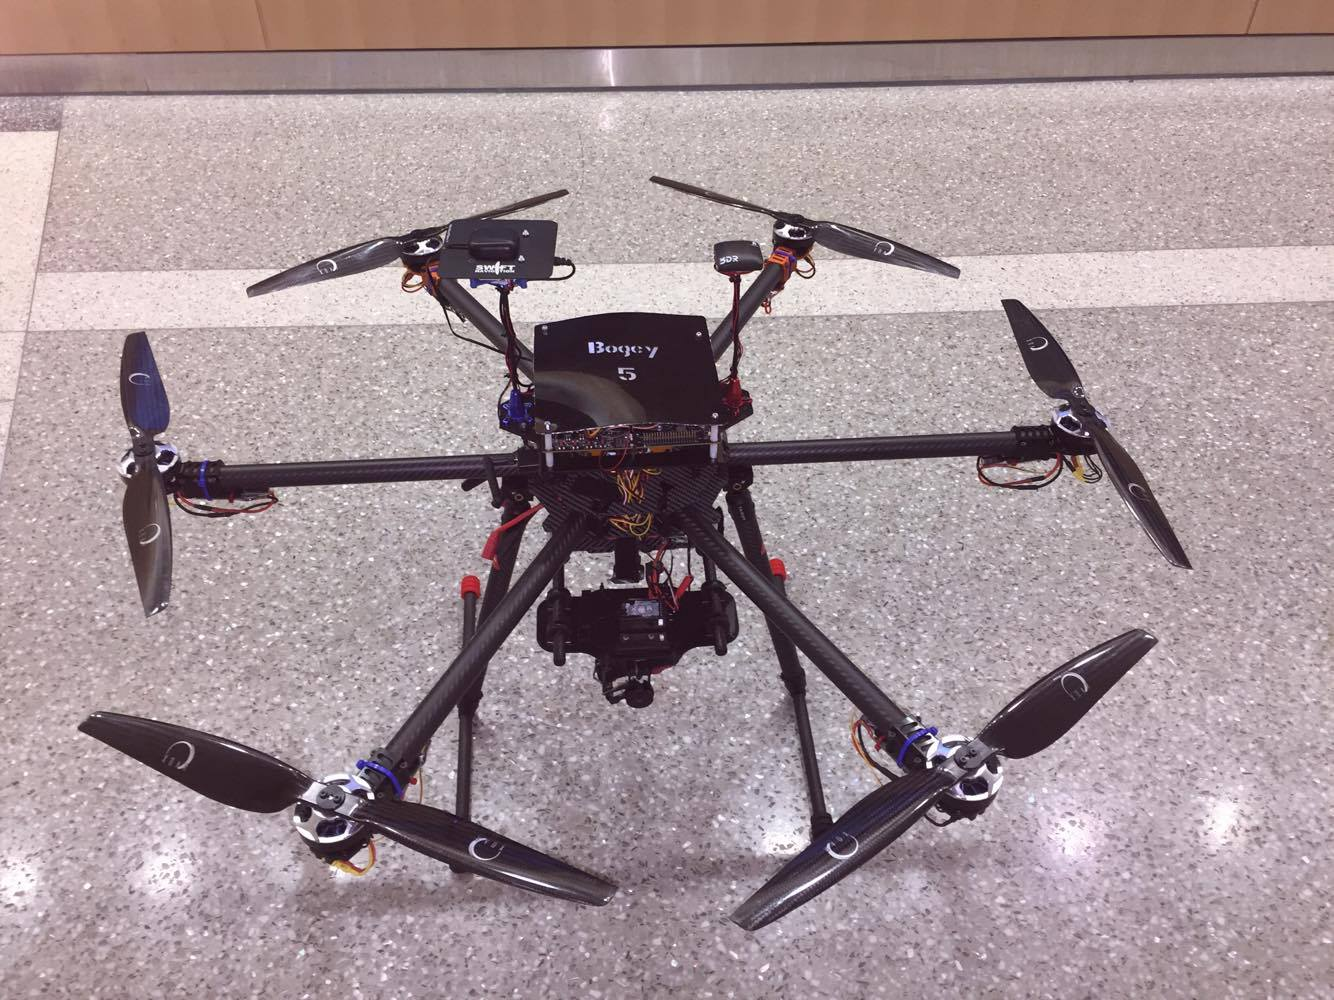
\includegraphics[width=1.0\textwidth,clip=true,trim=17 50 5 17]{images/bogey.jpg}
	\caption{Bogey : Autonomous Unmanned Aerial Vehicle Developed By Team VICTOR For MBZIRC 2017\label{bogey}}
\end{figure}

The Real Time Kinematic (RTK) GPS system was able to provide the 3D position of the UAV with respect to a base module setup in a fixed known point at an accuracy of 5cm. This accuracy was adequate for the UAVs to perform autonomous navigation in the context of the competition. However, the system required both the base module and the client module to have at least 5 satellites in sight, the communication between the base module and the client module was very susceptible to interferences and initialization of the system took time. Therefore a fall-back localization system was required to be implemented. As a result, a distance function based mapping and localization system was integrated to the UAV software stack to complement the RTK GPS based localization.\par

\subsection{Mapping The Environment}
To localize the UAVs, a map of the arena (a representation of the environment) was required to be built. The UAV was first navigated on a predefined path marked by waypoints using GPS data. During this flight, images were captured from the perspective camera. Typical images captured from the perspective camera are shown in figure \ref{arenaImagesPerspective}. Each image is first corrected for distortion and then stitched. The stitched image is then converted into a binary mosaic and the distance function is obtained after using an edge filter on the binary mosaic to represent the environment.\par

\begin{figure}
	\centering
	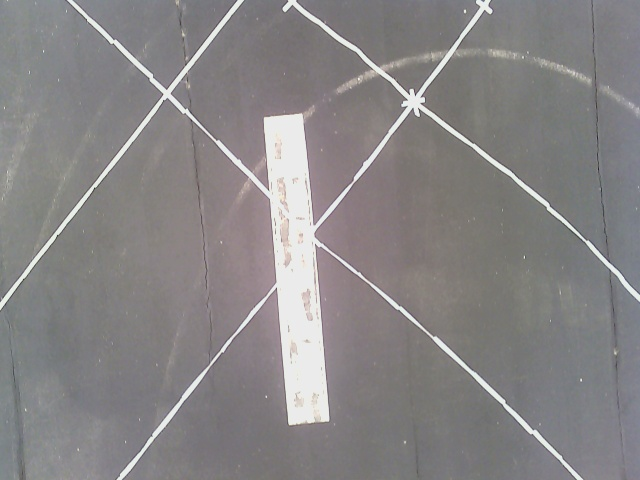
\includegraphics[width=0.80\textwidth,clip=true,trim=17 50 5 17]{images/kentland1.jpg}
    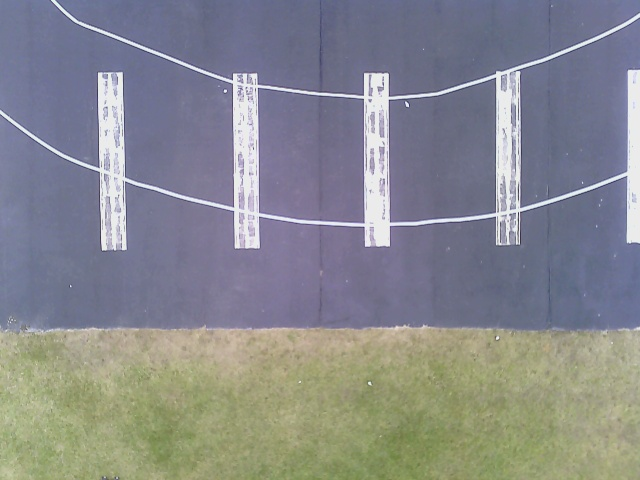
\includegraphics[width=0.80\textwidth,clip=true,trim=17 50 5 17]{images/kentland2.jpg}
	\caption{Typical images of the arena captured from the perspective camera\label{arenaImagesPerspective}}
\end{figure}

\subsection{Observing The Environment In Flight}
During flight, the images are captured from both the perspective camera and the fish-eye camera at 30 Hz frequency. The images are then corrected for distortion using pre-calibrated distortion parameters. The edges are extracted using an edge extractor after converting the 4-channel images to binary images. The extracted edges are then fed into the optimizer to calculate the corresponding pose for each image. It should be noted that the UAV platform is equipped with both a perspective camera and a fish-eye camera because, while the perspective camera can produce high resolution images of the ground plane, at low altitudes it doesn't have a large enough field of view to capture a significant area of the ground plane. A threshold was set at 5m and the perspective images were processed only when the single point laser range finder sensor reports an altitude above that threshold. When the UAV was flying low, only the fish-eye images were processed. 

\subsection{6-DOF Optimizer}
The final pose of the UAV (x, y, z, roll, pitch, yaw) was then calculated using an optimizer to match the captured image with the map previously built. The Chamfer distance between the map and the captured image was minimized using the Nelder-Mead algorithm \cite{nelder1965simplex} to find the optimal pose. This approach is required an initial guess which was provided using the Piksi RTK GPS and the IMU readings. The alternative was to do random sampling which was computationally too expensive to be implemented on this real-time system. 

\subsection{System Implementation And Pose Transformations}
The UAV was controlled using the Pixhawk\texttrademark flight controller. The high level tasks such as localization were executed on the on-board NVIDIA\texttrademark Jetson TX1 ARM processor. The communication between the two computers were carried out using MAVROS protocol and the system was implemented using the ROS framework.\par

\begin{figure}
	\centering
	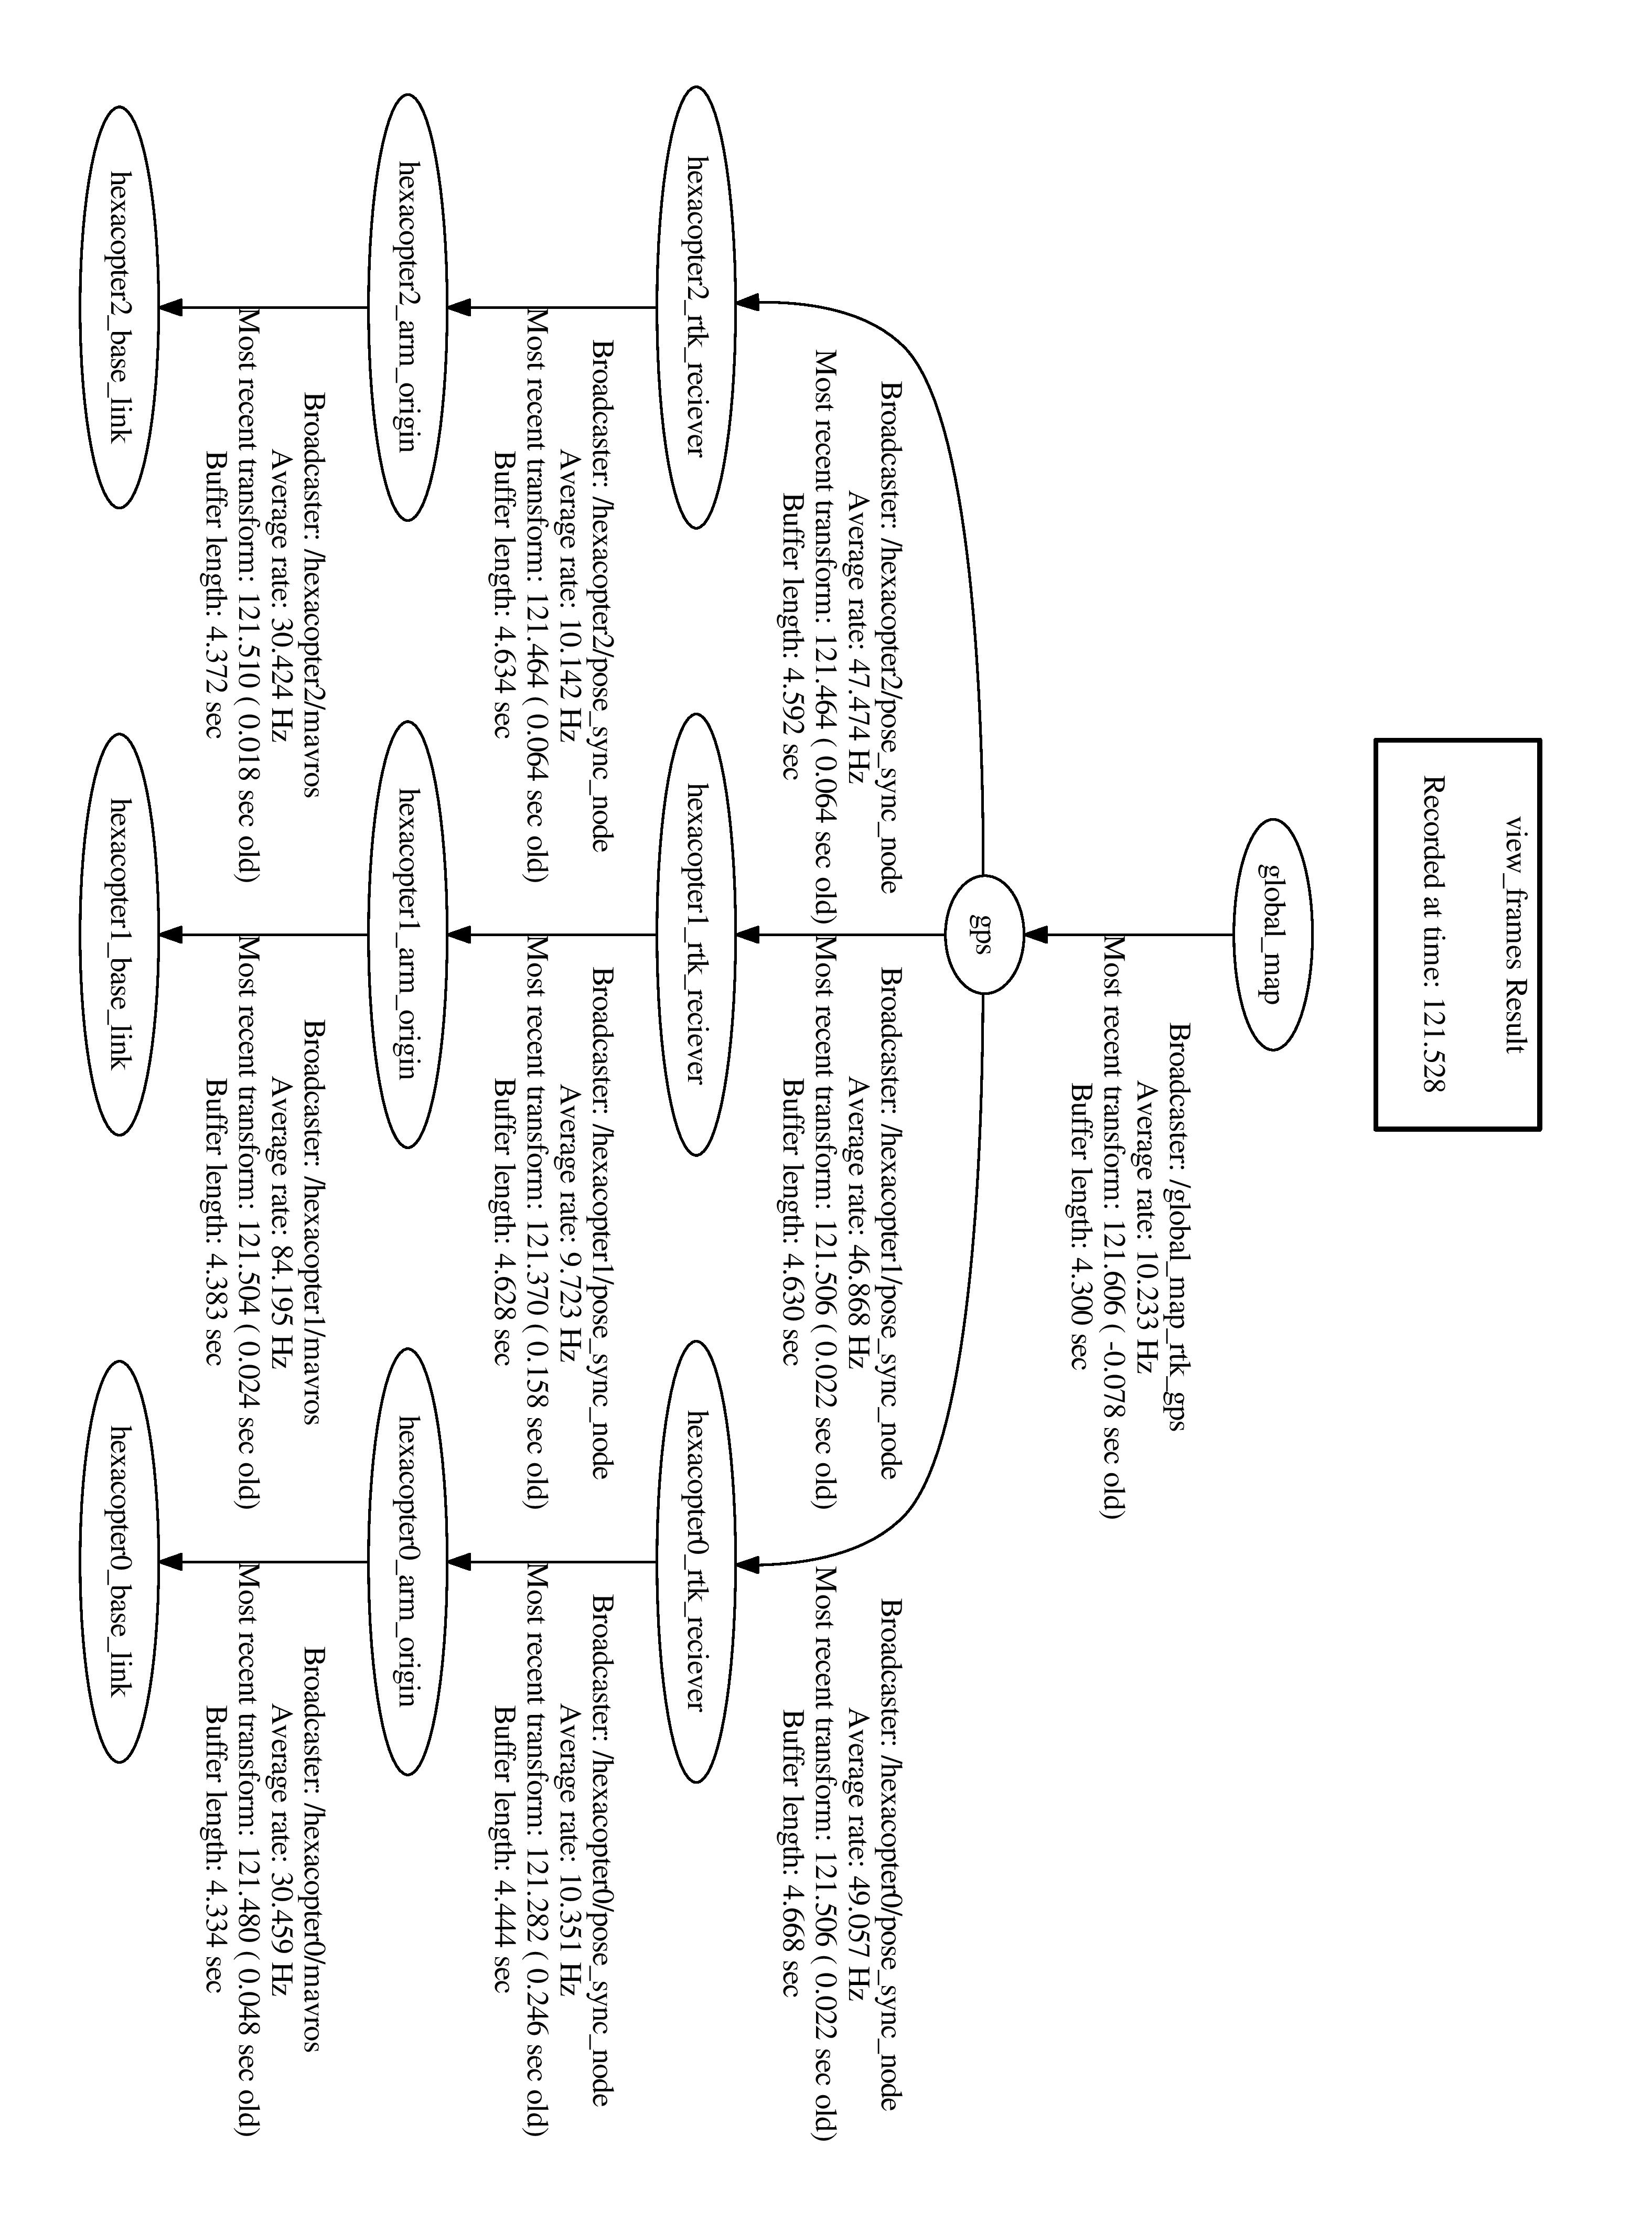
\includegraphics[width=1\textwidth,clip=true,trim=17 50 5 17]{images/tf-frames.jpg}
	\caption{Pose transformation of all three UAVs in simulation\label{tf_3UAV}}
\end{figure}

While the RTK GPS provides the position of the UAV with respect to a stationary base station, the distance function based localizer provides the pose of the UAV with respect to a global origin defined in the map. Transformation between the two coordinate systems was made simple by the ROS TF package which computes real-time synced pose transformations. Figure \ref{tf_3UAV} shows the UAV pose transformation implementation for challenge 3.

\section{Quadrotor Platform Simulation}
\label{platformSimProgress}
A novel robot platform was designed with the aim of giving it the ability to robustly navigate in highly cluttered and unstructured indoor environments to aid exploration of environments that are either unsafe or too small for humans move around in. The key ideas behind this design are listed here.

\begin{itemize}
\item Should be able to navigate in highly cluttered and unstructured indoor environments autonomously
\item Should have the capability to roll on surfaces including climbing walls
\item Should be able to tolerate impacts on surfaces
\end{itemize}

Intuitively, humanoid robots and wheeled robots are not good at navigating in unstructured and cluttered environments. With 6-DOF movement capability, UAVs, specially MAVs have better agility to move in such environments. However, the traditional UAV platform is not resilient to even the smallest collision against a solid surface, which is an inherent risk of navigating in such unstructured and cluttered environments. Therefore we propose a modification to the traditional UAV platform by introducing a light weight two wheel cage around the UAV. This modification allows the platform not only to fly in the space but also to roll around on planar surfaces.\par

Section \ref{litWallClimbingRobots} describes some approaches researchers have taken to develop robots that can move along vertical surfaces. In contrast, our platform can move not only on planar surfaces but in open space as well. Also, our platform is much smaller in size which makes it more suitable for navigation in unstructured and cluttered indoor environments. \par

The novel platform is designed and tested in a simulation environment as a proof of concept. The progress up to now is described in the following subsections. Section \ref{simulationEnvironment} gives a brief overview about the simulation environment. Section \ref{platformDesign} describes the platform design decisions. Section \ref{propellerSimulation} explains how the propellers were simulated. Section \ref{control} introduces the control strategies implemented in the simulation.

\subsection{Simulation Environment}
\label{simulationEnvironment}
The UAV platform is simulated using Gazebo, a free and open source robot simulation tool. The default Open Dynamics Engine (ODE) physics engine was used to model physics of the environment. The custom robot model is described using SDF and fed into the Gazebo. Custom plugins were implemented and attached to the robot model SDF to simulate propellers and control the robot.   

\subsection{Platform Design}
\label{platformDesign}
Figure \ref{quad_sim} shows the agile quadrotor platform simulated in the gazebo. The base of the platform where the UAV controller, the sensors and the batteries will be is modeled using a sphere for generalization. Three axes are fixed to the base where two of them will support the motors and the propellers and the third will connect the wheels. All dimensions, masses and moments of inertia are parameterized such that a change of material used for any component can be reflected in the simulation. The total mass of the current model is 66.5g. This is a reasonable value as a commercially available quadrotor with a cage was found to weigh 67g. 

\begin{figure}
\centering
	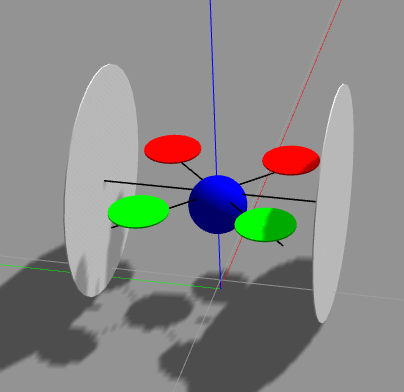
\includegraphics[width=1\textwidth,clip=true,trim=17 50 5 17]{images/simulation}
	\caption{Wheeled Quadrotor in Simulation\label{quad_sim}}
\end{figure}

\subsection{Propeller Dynamics Simulation}
\label{propellerSimulation}
While Gazebo can be used to simulate the physical world, it doesn't provide models for motors or propellers. To address this limitation, a quadrotor propeller system was implemented as a plugin to the system using the University of Illinois Urbana-Champaign (UIUC) propeller data set \cite{brandt_deters_ananda_selig_2017}.\par

The thrust force and torque generated by a propeller can be modeled by the expressions \ref{thrustEqn} and \ref{torqueEqn}.\par

\begin{equation}
\label{thrustEqn}
T = C_{T} \rho n^2  D^4
\end{equation}

\begin{equation}
\label{torqueEqn}
Q = C_{Q} \rho n^2 D^5
\end{equation}

\(\rho\) is the density of the air. n is the propeller speed in rps. D is the propeller diameter. The \(C_{T}\) and \(C_{Q}\) values are available for many propellers in the UIUC dataset. In the simulation, GWS 4x4 propellers (4 inch diameter, 4 inch pitch) are modeled using the UIUC data and expressions \ref{thrustEqn} and \ref{torqueEqn} with the \(C_{T}\) and \(C_{Q}\) values approximated using linear regression. The data set was verified using a propeller static thrust estimator. The use of a linear regression model to approximate the \(C_{T}\) and \(C_{Q}\) values is justified as in normal operating frequencies, they behave almost linearly with propeller speed.\par 

Once the thrust force and the torque generated by each propeller are calculated for the current propeller speeds, they can be applied on the model in the simulation directly.\par

\subsection{Control Strategies}
\label{control}
The quadrotor platform is controlled using the four motors \(M_{1}\), \(M_{2}\), \(M_{3}\) and \(M_{4}\). Each motor rotates the connected propeller to generate a thrust force and a torque which in turn controls the linear and angular accelerations of the platform.In a right handed coordinate system where it faces the positive direction of x axis, the thrust forces are always applied in the positive z direction. The torques from motors in the same axis are applied in the same direction and in the opposite direction of the torques applied by its two adjacent motors. \par

To move in the positive x direction, the quadrotor needs to pitch forward. The linear acceleration in the x direction is controlled by the thrust component in that direction, which depends on the thrust force generated by each propeller as well as the pitch angle. The angular acceleration about the y axis is controlled by the moment generated by the thrust differences between the forward motors and the rear motors. The yaw rate is controlled by the effective torque produced by the four propellers.\par

The first iteration of the platform controller was implemented ignoring the propeller dynamics for the sake of simplicity as shown in the expressions \ref{control1Motor1Force}, \ref{control1Motor3Force} and \ref{control1torque}.\par

\begin{equation}
\label{control1Motor1Force}
F_{1} = F_{2} = F_{c}
\end{equation}

\begin{equation}
\label{control1Motor3Force}
F_{3} = F_{4} = k_{1}(\theta_{d} - \theta) + F_{c}
\end{equation}

\begin{equation}
\label{control1torque}
T = k_{2}(-\psi)
\end{equation}

\(F_{i}\) denotes the thrust force applied on the platform by each propeller and T denotes the effective torque. \(\theta_{d}\) is the desired pitch and \(\theta\) is the actual pitch. \(\psi\) denotes the actual yaw angle of the platform. Since we want the quadrotor to move in the positive x direction, the desired yaw is set to 0. \(k_{1}\) and \(k_{2}\) were obtained by tuning the controller experimentally. 

However, this simple controller ignores one fundamental fact. The thrust force and the torque generated by a propeller are both functions of the propeller speed and thus they are not independent. Therefore in the second iteration, the propeller dynamics described in the subsection \ref{propellerSimulation} were used to design a controller as shown in the expressions \ref{control2velocityAngle} to \ref{control2w4}. 

\begin{equation}
\label{control2velocityAngle}
\theta_{d} = kv_{x}(v_{xd} - v_{x})
\end{equation}

\begin{equation}
\label{control2velocityRotation}
\Delta\omega_{x} = k_{pp}((\theta_{d} - \theta) - k_{pd}\ v_{p})
\end{equation}

\begin{equation}
\label{control2yaw}
\Delta\omega_{\psi} = k_{\psi p}((-\psi) + k_{\psi d}\ v_{\psi})
\end{equation}

\begin{equation}
\label{control2w1}
\omega_{1} = \omega_{c} + \Delta\omega_{\psi}
\end{equation}

\begin{equation}
\label{control2w2}
\omega_{2} = \omega_{c}
\end{equation}

\begin{equation}
\label{control2w3}
\omega_{3} = \omega_{c} + \Delta\omega_{x} + \Delta\omega_{\psi}
\end{equation}

\begin{equation}
\label{control2w4}
\omega_{4} = \omega_{c} + \Delta\omega_{x}
\end{equation}

The propeller speeds for each motor \(\omega_{1}\), \(\omega_{2}\), \(\omega_{3}\) and \(\omega_{4}\) are calculated using the desired velocity in x direction (\(v_{xd}\)) and desired yaw set to 0. \(v_{x}\) is the robot's velocity in z direction. \(v_{\psi}\) is the angular velocity of the robot about Z axis. Constants \(kv_{x}\), \(k_{pp}\), \(k_{pd}\), \(k_{\psi p}\) and \(k_{\psi d}\) were obtained by tuning the controller experimentally.\par

Once the propeller speeds are calculated, the resulting forces and torques are calculated using expressions \ref{thrustEqn} and \ref{torqueEqn} and are applied on the platform in the simulation.

\bibliographystyle{ieeetr}
\bibliography{bibliography}

\end{document}